%%%%%%%%%%%%%%%%%%%%%%%%%%%%%%%%%%%%%%%%%
% UQ AWMC Document Template
% LaTeX Template
% Version 1.0 (27/12/12)
%
% This template has been downloaded from:
% http://www.LaTeXTemplates.com
%
% Original author:
% WikiBooks (http://en.wikibooks.org/wiki/LaTeX/Title_Creation)
% Modified by Ed Barry for UQ.
% License:
% 
%----------------------------------------------------------------------------------------
%	PACKAGES AND OTHER DOCUMENT CONFIGURATIONS
%----------------------------------------------------------------------------------------


\documentclass[12pt]{article}
%\usepackage[french]{babel}
\usepackage[utf8x]{inputenc}
\usepackage{amsmath}
\usepackage{graphicx}
\usepackage{float}
\usepackage{dsfont}
\usepackage{amsfonts}
\usepackage[T1]{fontenc}
\usepackage[colorinlistoftodos]{todonotes}
\usepackage{listings}
\setlength{\parindent}{0pt}
\newcommand{\deriv}{\mathrm{d}}
\lstset{
    language=octave,
    basicstyle=\scriptsize\ttfamily,
    commentstyle=\ttfamily\color{red},
    numbers=left,
    numberstyle=\ttfamily\color{blue}\footnotesize,
    stepnumber=1,
    numbersep=5pt,
    backgroundcolor=\color{white},
    showspaces=false,
    showstringspaces=false,
    showtabs=false,
    frame=single,
    tabsize=2,
    captionpos=b,
    breaklines=true,
    breakatwhitespace=false,
    title=\lstname,
    escapeinside={},
    keywordstyle={},
    morekeywords={}
    }

\title{Introduction to Scientific Computing using MATLAB}

\begin{document}

\begin{titlepage}

\newcommand{\HRule}{\rule{\linewidth}{0.5mm}} % Defines a new command for the horizontal lines, change thickness here

\center % Center everything on the page
 
%----------------------------------------------------------------------------------------
%	HEADING SECTIONS
%----------------------------------------------------------------------------------------

\textsc{\LARGE CHEE2010}\\[1.5cm] % Name of your university/college

\includegraphics[scale=1.2]{awmc.jpg}\\[1cm] % Include a department/university logo - this will require the graphicx package

\includegraphics[scale=0.3]{uq.jpg}\\[1cm]
\textsc{\Large }\\[0.5cm] % Major heading such as course name

%----------------------------------------------------------------------------------------
%	TITLE SECTION
%----------------------------------------------------------------------------------------

\HRule \\[0.4cm]
{ \large \bfseries Introduction to Scientific Computing using MATLAB}\\[0.4cm] % Title of your document
\HRule \\[1.5cm]
 
%----------------------------------------------------------------------------------------
%	AUTHOR SECTION
%----------------------------------------------------------------------------------------

\begin{minipage}{0.4\textwidth}
\textit{Authors:}\\Edward \textsc{Barry} \\ Felix \textsc{Egger}\\ % Your name


\end{minipage}\\[2cm]

%----------------------------------------------------------------------------------------
%	DATE SECTION
%----------------------------------------------------------------------------------------


\end{titlepage}

\tableofcontents

\newpage

\section*{General Introduction}
Many of the courses through this degree will involve numerical computing and operations on large sets of data. You will have have the choice of using spreadsheet tools such as MS Excel, or using scripting languages such as Matlab to complete this course. This document aims to make the latter more appealing.\\


When you write your scripts, please suppress outputs to the console using the \texttt{;} (semicolon) symbol. They can quickly get very annoying. If you would like to display the results of a calculation to the console, store it as a variable, and display the variable with the \texttt{disp(variable)} command. \\

The percentage symbol \texttt{\%} indicates a comment. The Matlab interpreter will not process anything written after the percentage symbol. It is important to add comments to your scripts, but the best written scripts should not need much commenting, as the code will speak for itself. It is up to you to find a happy medium in your commenting conventions. Generally, it is bad practice to comment on the syntax of the programming language, but good practice to clarify what is expected of a certain block of code. 

\begin{lstlisting}
%"""Bad commenting practice"""
% create an index i, and loop through each element of the array A checking if each element is odd or even, then print it out to the console
for i = 1:length(A)
	if mod(A(i), 2) == 0
    	disp(A(i));
    end
end


%""" More bad commenting """
% Calculate the area of a circle
R = 1.2
A_circle = pi  * R.^2
\end{lstlisting}

Lastly, this is not an exhaustive guide, it just covers the basic functionality of the Matlab environment. If you forget how to use certain functions in Matlab, the \texttt{doc} keyword will be of aid. Calling \texttt{doc <subroutine>} (where <subroutine> is the name of an inbuilt Matlab function) directs you to a new window where you can learn about the function, and how to implement it. For example, typing
\begin{lstlisting}
doc length
\end{lstlisting}
brings up the documentation for the function \texttt{length}, its usage and similar functions that might be useful for the task you are trying to perform.

%----------------------------------------------------------------------------------------
%	Navigation and Naming conventions
%----------------------------------------------------------------------------------------
\section{Navigation}
Navigating around the Matlab development environment can be a bit daunting at the start. There are a number of rules that we need to follow to make the process as seamless as possible.
\subsection{Navigating to appropriate directory}
When you are carrying out operations on datasets or are using custom functions, you need to ensure that the Matlab interpreter knows where these datasets are. Navigate to the folder you want to work in by selecting it down the left hand side of the window (Figure \ref{fig:mde}). \\
\begin{figure}[ht]
\centering
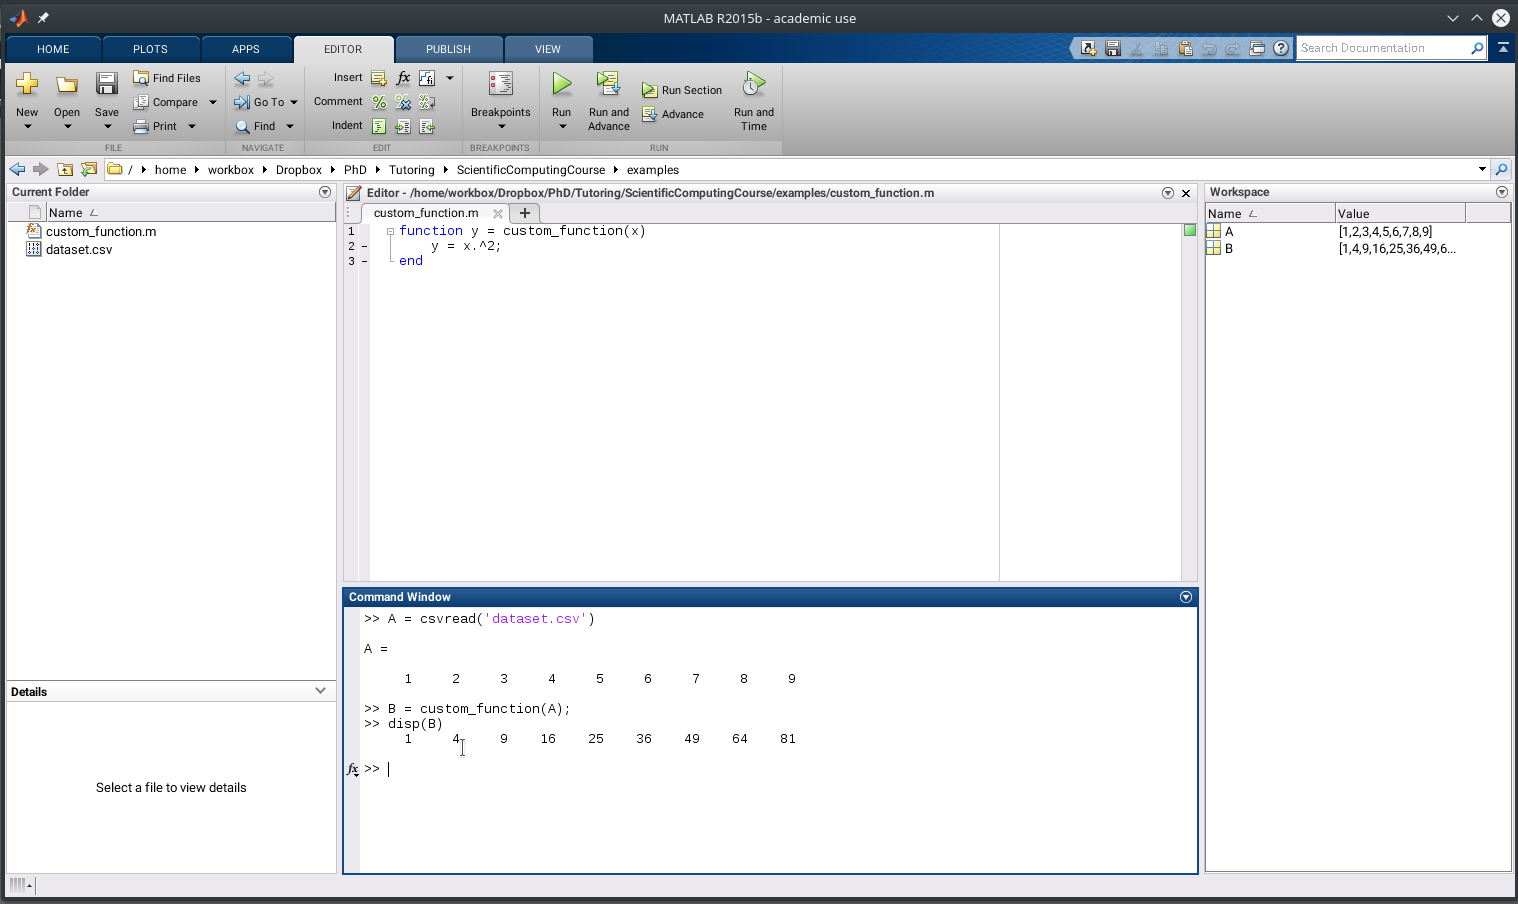
\includegraphics[scale=0.4]{navigation.png}
\caption{Main Matlab development environment}
\label{fig:mde}
\end{figure}

Down the left hand side, we have navigated to the directory which includes the function \texttt{custom\_function.m} and the dataset called \texttt{dataset.csv}. If we change directories and try to run the commands in the command window, we will get an error message (Figure \ref{fig:mde2}).\\
\begin{figure}[ht]
\centering
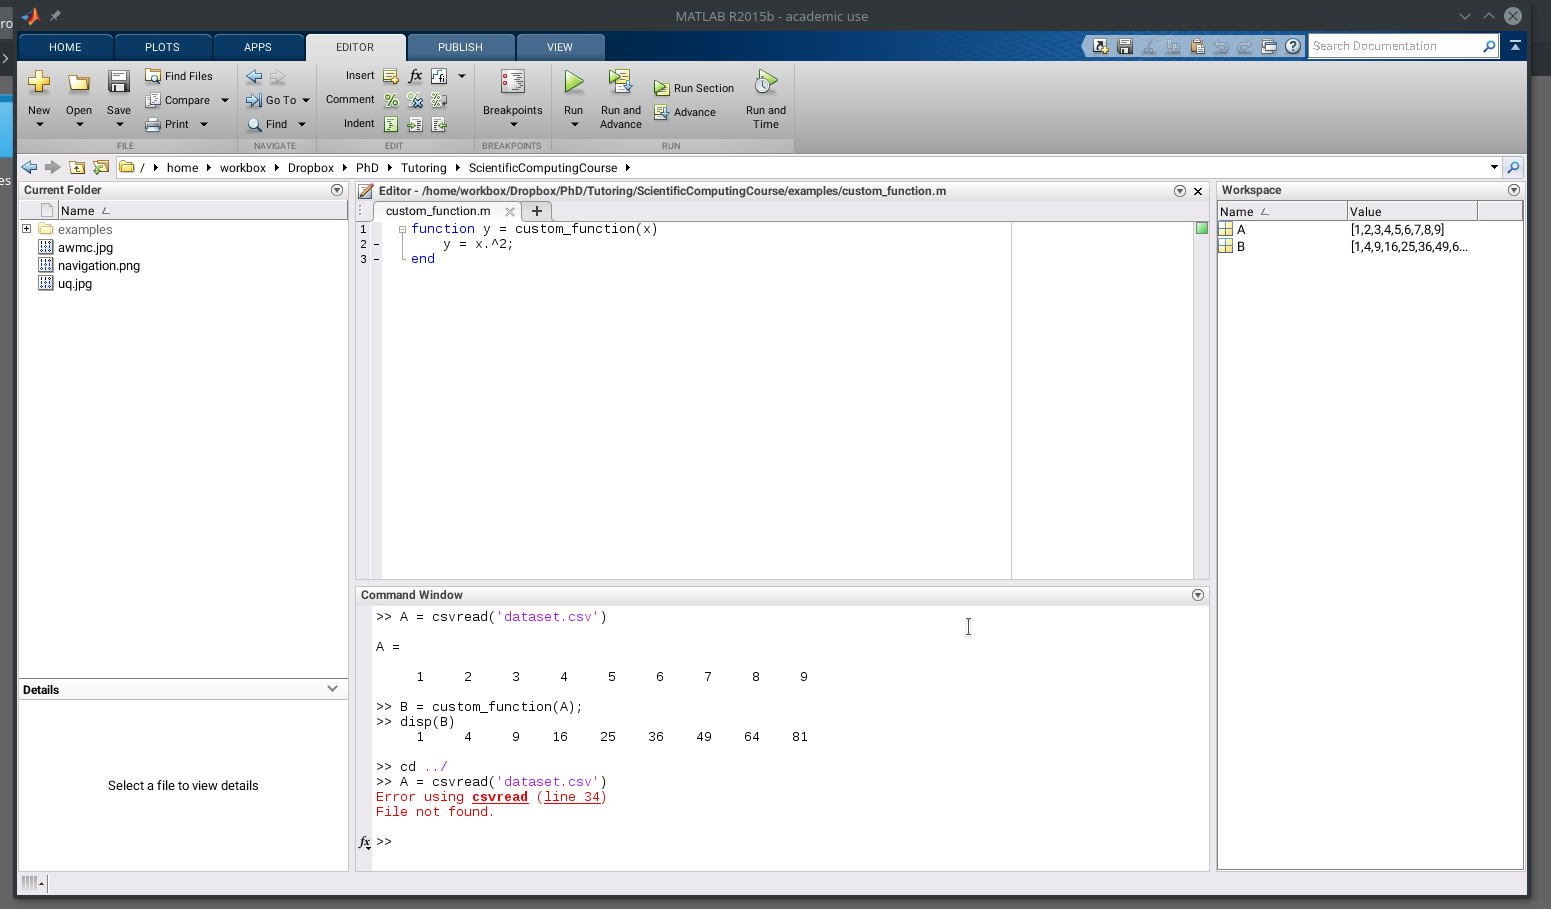
\includegraphics[scale=0.4]{navigation2.png}
\caption{Demonstration of error message if we are not in the right working directory.}
\label{fig:mde2}
\end{figure}

Matlab comes with many built-in functions and we can use these highly optimised routines to carry out our scientific computing tasks. For example, if we want to calculate the scalar dot product of two tensors (scalars, vectors, matrices), we don't need to navigate to the directory where this function/routine exists. The Matlab interpreter knows where its standard functions are located. Rather than writing your own basic functions, you should take advantage of what Matlab developers have already done. For more information about what is available in Matlab, please visit \texttt{https://au.mathworks.com/help/matlab/.}

\subsection{Naming conventions}
When you create a new script, make sure the script is logical and pertinent to its specific task. For example, in the function written previously, \texttt{custom\_function.m} is not particularly insightful. You can see that the function takes input and squares it, so why not call it something like \texttt{square.m}? That said, \texttt{custom\_function.m} is much better than the default \texttt{Untitled.m}. Many students fall into this trap, and struggle to keep track of their workflow. A good way to combat this is to create files from the command window, rather than create them graphically. Suppose we want to create a function that calculates the settling velocity of a particle in a fluid (\texttt{settlingVelocity.m}. We can do this using the edit function. If the file exists, it will take us to the file editor. If it doesn't exist, it will ask us if we want to create a new file with the file name \texttt{settlingVelocity.m} (Figure \ref{fig:edit_command}).

\begin{figure}[ht]
\centering
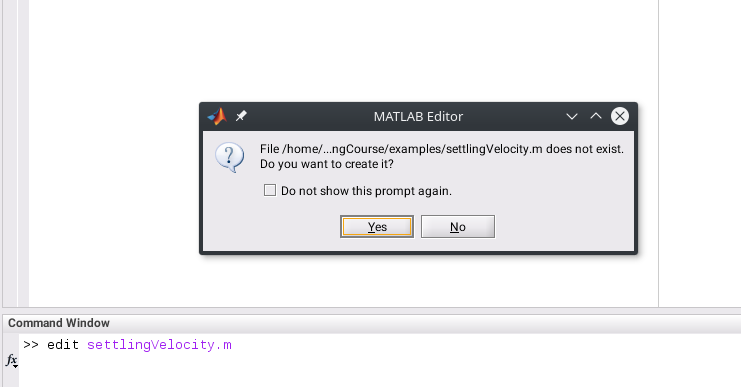
\includegraphics[scale=0.8]{touch.png}
\caption{Example of the \texttt{edit} command in Matlab.}
\label{fig:edit_command}
\end{figure}




%----------------------------------------------------------------------------------------
%	Data Types
%----------------------------------------------------------------------------------------
\newpage
\section{Data types}
Data types are an important concept in computer science. The design of the Matlab language means that we don't have to worry too much about data types, but it's always good to keep these things in mind. The data types most useful to us in Matlab are:
\begin{itemize}
\item \texttt{double} : double precision floating point (look it up)
\item \texttt{bool} : boolean true or false
\item \texttt{char} : characters (single dimension) and strings of characters (multidimensional)
\end{itemize}

To determine all the information available for your current working variables, the command \texttt{whos} is your friend.\\

\textbf{N.B.} all numerical variables are of type \texttt{double} in Matlab. The data type \texttt{double} can have different dimensions, and we will see what that means when we look at Section \ref{sec:tensors}. Double precision floating point numbers are real numbers occupying 64 bits of space (single precision floating point is a 32 bit real). This means that we can have precision to about 16 decimal places. Therefore, if you compute a function that returns a value of $10^-20$, it is no different from zero. 


%----------------------------------------------------------------------------------------
%    READING AND WRITING FILES 
%----------------------------------------------------------------------------------------
\section{Reading and Writing Files}
Dealing with data files is important in a course like CHEE2010. After all, this is all about data analysis, and we sometimes operate on big sets of data. \\

\subsection{File types}
There are a couple of file types that we should stick to when doing data analysis:
\begin{itemize}
\item \texttt{*.csv}
\item \texttt{*.txt}
\item \texttt{*.xls}
\end{itemize}

The first two file types are preferred to the \texttt{*.xls} file type, as the latter is compiled with a lot of metadata behind it. Additionally, if you have big jobs to send to computing clusters, the MS Excel format won't be recognised on these systems. However, for jobs done on your personal computer, playing with \texttt{*.xls} files should be fine. 

\subsection{Opening and Writing CSV files}
CSV files can be opened and created with the commands \texttt{csvread}, and \texttt{csvwrite}.
Let's say there's a file called \texttt{myDataFile.csv} in the same working directory as your Matlab script or workspace. To open this file, enter in the following command. 
\begin{lstlisting}
data = csvread('myDataFile.csv');

\end{lstlisting}
This saves the dataset as the variable \texttt{data}. If there are headers in the file, you can use row and column offsets in the following manner:
\begin{lstlisting}
row_number = 1;
col_number = 0;
data = csvread('myDataFile.csv', row_number, col_number);
\end{lstlisting}
The previous command will ignore the first row and start 1 row down. An error message will be thrown if you try to import non-numerical data with the \texttt{csvread} command.\\

In order to write an array to CSV, the command \texttt{csvwrite} is useful. The arguments passed into the function are, in order, \texttt{filename.csv}, \texttt{arrayName}, \texttt{row\_offset} and \texttt{col\_offset}. For example, we want to write matrix A to file \texttt{results.csv}. We want all rows and columns.\\
\begin{lstlisting}
csvwrite('results.csv', A, 0, 0);
\end{lstlisting}

\subsection{Opening and writing all files}
The routine \texttt{importdata} allows us to import many different file formats into a Matlab array. As the output is an array, we must only use this routine with numerical datatypes. There is one mandatory argument to pass into this function, \texttt{'filename.extension'}. Other optional arguments are \texttt{delimiterIn}, and \texttt{headerlinesIn}. If we have a text file which separates each column with spaces, and the first row consists of headers (non-numerical data), then to import a text file as an array \texttt{A}, we issue the following command:
\begin{lstlisting}
A = importdata('my_file.txt', delimiterIn=' ', headerlinesIn=1);
\end{lstlisting}

\subsection{Reading and writing MS Excel files}
To import data from \texttt{*.xls} files, the command is \texttt{xlsread}. There is one mandatory argument (\texttt{filename}), passed in as a string with extension. Optional arguments include \texttt{sheet} (for when you have multiple worksheets in the same file, \texttt{xlRange}, which is the range of the sheet you want, from top left to bottom right. \texttt{sheet} can be passed in as the index (sheet number from left to right), or as a string. \texttt{xlRange} is passed in as a string. Suppose we want to import data from the second sheet of an MS Excel file named \texttt{experiment\_results.xls}. We want all data from A2 to D24 (top left to bottom right). The data will be assigned to an array called \texttt{my\_xls\_array}.
\begin{lstlisting}
sheet = 2;
xlRange = 'A2:D24';
my_xls_array = xlsread('experiment_results.xls', sheet, xlRange); 
\end{lstlisting}

To write an array to MS Excel, \texttt{xlswrite} is the command. It accepts two mandatory arguments (filename with extension, as a string) and array name (as per Matlab workspace). Optional arguments are \texttt{sheet} which can be passed as a string or index (number). If the particular sheet does not exist, Matlab will create a new sheet. Finally, \texttt{xlRange} is passed as a string, and places the array in the corresponding coordinates in the \texttt{*.xls} file. If only specified as a single MS Excel cell, \texttt{xlRange} will use that value as the starting point for the array. Suppose we have an array A that we want to save as \texttt{calculated\_results.xls}, and we want our array to start at cell E4 of sheet 2.
\begin{lstlisting}
xlRange = 'E4';
sheet = 2;
xlswrite('calculated_results.xls, A, sheet, xlRange);
\end{lstlisting}

For more information, please see the Matlab documentation on how to deal with datafiles. \\
\texttt{https://au.mathworks.com/help/matlab/data-import-and-export.html}. Another method for importing data is using the graphical tool. Please prioritise the use of text methods for data import, as they are much easier to use in the long run. It is also good to avoid importing data graphically when you are submitting work for assessment. It's much easier if we receive a file that just works right off the bat. 

%---------------------------
%	SCALARS/ARRAYS/MATRICES 
%----------------------------------------------------------------------------------------
\section{Scalars, Arrays and Matrices (Tensors)}
\label{sec:tensors}

Matlab is based on tensor mathematics (hence the name \textbf{MATrix LABoratory}). We already have a good idea as to what a tensor is from the introductory maths courses taught at UQ. 

\subsection{Slicing Matrices}
There might be times where you need to take a subset, or slice from a matrix. Suppose you have a big set of time series data, and you are only interested in what happens at the final time step. Let's create a dummy matrix of periodic data and create a new variable with just the final time step.

\begin{lstlisting}
t = [0:1:20]';
A = [t, sin(t)];
final_step = A(end,:);
\end{lstlisting}

Now, suppose we only care about the initial condition:
\begin{lstlisting}
initial_step = A(1,:);
\end{lstlisting}

Now, lets take the state of the system at the halfway point
\begin{lstlisting}
% Search for the meaning of the routines ceil and length
midpoint = A(ceil(length(t)/2), :);
\end{lstlisting}
%----------------------------------------------------------------------------------------
%	Operators 
%----------------------------------------------------------------------------------------
\newpage
\section{Operators}
Operators tell the interpreter to manipulate variables in a certain way. For example, in mathematics, the operator \texttt{+} operates on two numbers, $a$, $b$ $\in$ $\mathbb{C}$ or any subset thereof, and returns the addition of $a$ and $b$. There are different types of operators in programming languages, and we will discuss only the most pertinent ones to the course.
\begin{itemize}
\item arithmetic operators
\item logical operators
\end{itemize}

\subsection{Arithmetic operators}
\subsubsection{+ operator}
The + operator works on tensors provided they are the same size and dimension. The exception to the rule is when one of the variables is a scalar, just like in mathematics. See the example in Figure \ref{fig:add} where we explore what can and can't be done with the addition operator in Matlab. 
\begin{figure}[ht]
\centering
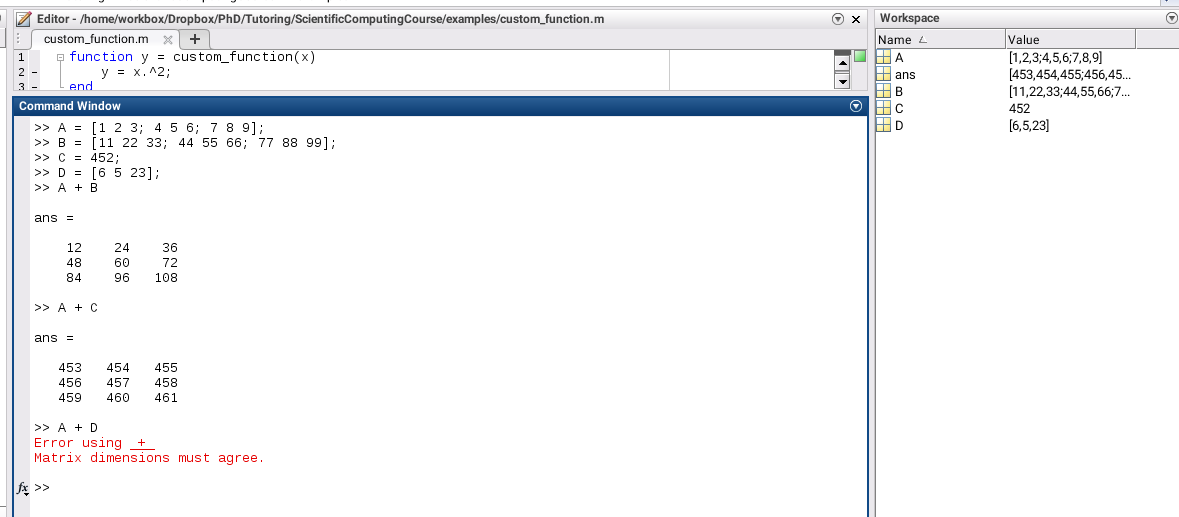
\includegraphics[scale=0.8]{add_operator.png}
\caption{Addition operator applied to matrices and scalars}
\label{fig:add}
\end{figure}


\subsubsection{- operator}
The - operator works in the same way as the + operator. Nothing to add. 

\subsubsection{* operator}
The \texttt{*} operator multiplies matrices together. Be careful, you must consider matrix operations when using this operator. If you want to multiply all elements of matrix A with the corresponding elements of matrix B, then you need to include a '.' directly before the \texttt{*} operator. Refer to Figure \ref{fig:mult} for an example of how the \texttt{*} and \texttt{.} operators are used. In this course, we rarely do matrix operations, so we will often be using the elementwise operator. Note the use of another operator in the example. The \texttt{'} transposes matrices which may be of use, especially when data is in row format, and you want to work with columns, or vice versa. 

\begin{figure}[ht]
\centering
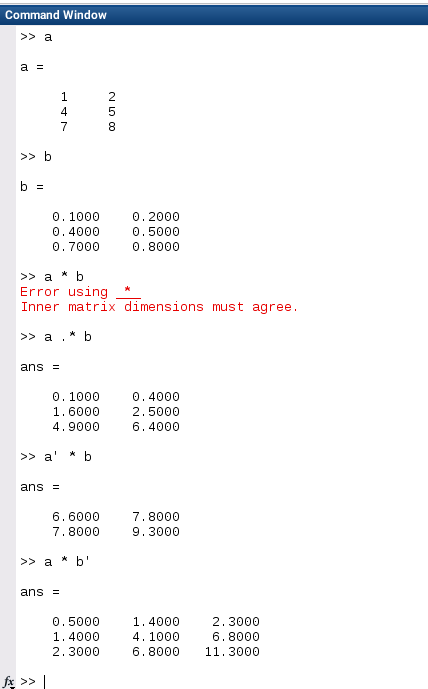
\includegraphics[scale=0.6]{mult_operator.png}
\caption{Multiplication and element-wise multiplication operators applied to matrices}
\label{fig:mult}
\end{figure}

\subsubsection{/ operator}
This works in a similar way to the \texttt{*} operator. 


\subsubsection{\texttt{\^} operator}
This is the power operator. You must be careful with this when dealing with matrices. It works as expected for scalars. If you want to play it safe, place the \texttt{\.} ahead of the \texttt{\^} to ensure element-wise exponents.

\subsubsection{\texttt{mod} operator}
\texttt{mod(a,b)} (modulo operator) returns the remainder when \texttt{a} is divided by \texttt{b}. This can be useful when checking if a number is even or odd. \textit{e.g.}
\begin{lstlisting}
mod(5,2) % returns 1 -> odd
mod(6,2) % returns 0 -> even
\end{lstlisting}

\subsubsection{= operator}
The assignment (\texttt{=}) operator allows us to store values of any data type to a variable name. For example, if we want to store the result of the multiplication of 6.2 and 8.029 to variable \texttt{a}, we use the assignment operator.
\begin{lstlisting}
a = 6.2 * 8.029 % -> a = 49.7798
\end{lstlisting}

\subsubsection{\texttt{@} (at) operator}
The \texttt{@} operator allows us to use functions as variables. This will be covered in more detail in Section \ref{sec:functions} (Functions). 

\subsection{Logical (boolean) operators}
Boolean operations are quite important in computer science. It allows us to check for conditions, and execute code if the condition holds or pass over the code if not. It is more useful than we expect.

\subsubsection{== operator}
This returns 1 if true, and 0 if not. Note the double equals sign. The single equals sign is for variable assignment. 
\begin{lstlisting}
a = 22;
b = 33 - 11;
a == b % -> true
c = pi;
a == c % -> false
\end{lstlisting}

\subsubsection{Other logical operators}
\begin{itemize}
\item \texttt{>} (greater than)
\item \texttt{>=} (greater than or equal)
\item \texttt{<} (less than)
\item \texttt{<= }(less than or equal)
\item \texttt{{\raise.17ex\hbox{$\scriptstyle\mathtt{\sim}$}}=} (not equal)
\end{itemize}

Suppose we have an array of temperatures over a 12 month period. We want to check how many days had a maximum of over 30.0 C. The daily maxima from the Bureau of Meterology for 2017 were downloaded for this exercise. \\ (\texttt{http://www.bom.gov.au/climate/data/}). \\


\begin{lstlisting}
temps = csvread('bom_2017_temp.csv', 1, 1);

%How many days per month had a max over 30 C?
days_per_month = sum(temps > 30.0);

%How many total days in the year?
days_per_year = sum(days_per_month > 30.0);
\end{lstlisting}

For each element in temps, if the temperature is over 30.0 C, the boolean \texttt{>} operator returns a 1, and we compute the sum of all the positive results. It is the same process for the number of days in the year. From these quick commands, we find that 93 days had a maximum temperature greater than 30 degrees in 2017.

%----------------------------------------------------------------------------------------
%	Functions
%----------------------------------------------------------------------------------------
\newpage
\section{Functions}
\label{sec:functions}
Globally, functions take arguments as input, perform a bunch of operations on these inputs, and return output arguments to the workspace or console. In other computing languages and paradigms, functions are known as routines, subroutines, or class methods. We will discuss two types of functions in this section: lambda functions, and function files. 

\subsection{Lambda functions}
Lambda functions, or anonymous functions, are defined in a script, and are only defined within that script. You can't access these functions from another script. The advantage of these functions is that we can maintain a relatively simple project, and we don't have many different function files written for a whole bunch of small tasks. It basically helps with workflow. If the functions become more unwieldy, it is better to write a dedicated function file. Suppose we have a vector or time values, and we want to apply a periodic function to these values. The lambda function, that we will call \texttt{periodic\_fct} is defined in the following manner:
\begin{lstlisting}
periodic_fct = @(x, A, C, D) A * sin(t*C) + D;

A = 4.21;
C = 10;
D = 20;
t = 0:0.1:10;
y = periodic_fct(t);
plot(t, y);
\end{lstlisting}
Do you notice that when we define the time vector in the lambda function, it is defined as \texttt{x}, but when we use it for computation, we pass \texttt{t} into the function. This is fine, it doesn't matter what the variables are called, it just matters that each variable goes in the appropriate order when applying the function. This holds for normal functions as well.

\subsection{Function files}
When functions are either complex and specialised or simple and very generic, it is usually a good idea to write a function file. Below is an example of how a function file is set up. This is a standalone file, and not written within any other script. When saving the file, it's good practice to save it as the name of the function, in this case, \texttt{sphere\_dimensions.m}.
\begin{lstlisting}
function [d, sa, V] = sphere_dimensions(r)
		d = 2 .* r;
    sa = 4 * pi .* r .^ 2;
    V = 4 * pi .* r .^ 3 / 3;
end
\end{lstlisting}

Firstly, the \texttt{function} keyword is required. The second term \texttt{[d, sa, V]}, is the list of outputs. You can specify as many outputs as you like in the form of an array. The first term on the right hand side of the equation is the name of the function. When calling functions from the script, this is the term to use. Within the brackets are the input arguments. They must be called in the right order in the script. When calling the function in the script, it doesn't matter what the input or output arguments are called, it just matters that they are in the right order. Below is an example of calling \texttt{sphere\_dimensions} from a script file.\\
\begin{lstlisting}
R1 = 32;
R2 = 64;
[diam1, surf_area1, volume1] = sphere_dimensions(R1);

[diam2, surf_area2, volume2] = sphere_dimensions(R2);
\end{lstlisting}

Again, as we see in the example, it does not matter what we call the arguments in or out of the function, but it does matter that the argument in is a radius, and that the arguments out are diameter, surface area and volume respectively. The input arguments can be passed in as an array of any dimension, but be careful of your matrix operators. See if you can condense the previous script, passing in the two radii as an array of radii. 
%----------------------------------------------------------------------------------------
%	Loops
%----------------------------------------------------------------------------------------
\newpage
\section{Loops}
When you want to avoid doing the same thing over and over again, a loop is often a solution. In Matlab, you have the option of writing \texttt{for} loops and \texttt{while} loops. Oftentimes, we are checking if some certain condition is true and executing code if so.

\subsection{\texttt{for} loops}
Let's write a \texttt{for} loop which checks if each element in an array is even, then prints those numbers to the console.

\begin{lstlisting}
% Define an array with random integers
A = ceil(10*rand(100,1));

for i = 1:length(A)
	if mod(A(i), 2) == 0
    	disp(A(i)); disp(i);
    end
end
\end{lstlisting}
What this loop does is start from i = 1, and checks if the first element of A is even. If A(1) is even, then we print the number to the console, as well as where in the array the even number is located. If A(i) is odd, then nothing is done, and we move onto A(i + 1). This repeats for the whole length of A. 

\subsection{\texttt{while} loops}
While loops have an inherent boolean nature. They continue to execute code while a certain statement is true. Once the statement becomes false, the loop breaks and we move onto the next bit of code in the program. Let's write a \texttt{while} loop which calculates the following series and tells us for what value of $n$ the sum exceeds $100$
\begin{equation}
S_n = \sum_{k=1}^{n} \frac{1}{\sqrt{k}}
\end{equation}
\newpage
\begin{lstlisting}
S = 0; k = 0;

while S <= 100
	k = k + 1;
	S = S + 1 / sqrt(k); 
end

disp(k);
\end{lstlisting}
As is clear from the loop, the code keeps executing while the value of S is not greater than 100. Once this statement does not hold true, the loop exits and we print the last value of k. 
%----------------------------------------------------------------------------------------
%	Workflow
%----------------------------------------------------------------------------------------

\section{Workflow}
Functions and scripts are two different things. Functions are written so that routines can be packaged up and reused when we like. Scripts are where all the manipulation is done. We use scripts to define the actual parameters of our work, to call functions, to manipulate the values of variables, to read and write to files, and to plot our results. The script where we define all of these things is often called a driver file. It is important that we understand the distinction between these two file types. Figure \ref{fig:sym} shows two files in the current folder. The icon next to the file name shows you what type of file it is. The \texttt{fx} on the icon shows you that this file is a function and the Matlab logo on the icon shows you that the file is a script. Note that both files have the file extension \texttt{*.m}.
\begin{figure}[ht]
\centering
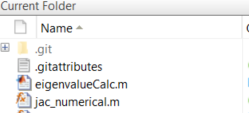
\includegraphics[scale=1]{file_symbols.PNG}
\caption{File types in the current folder}
\label{fig:sym}
\end{figure}

\section{Plotting}
Plotting can be carried out in a much quicker than in MS Excel. Another advantage is that once we have a design that looks good, we can reuse those settings for subsequent graphs without too much effort.\\
Most of the help with plotting can be found using your browser, however, we will cover the most basic types of plots we will use. The boxplot of summer temperatures by month can be seen in Figure 6.

\begin{lstlisting}
% We have t and y defined, and want a scatter plot of red asterisks
figure(1)
plot(t, y, 'r*')
xlabel('time (s)')
ylabel('concentration (M)')
title('Concentration of reagent Y over time')



% We have an array of temperature values for the last 10 Januarys, we want a historgram of their distribution
temperatures = norminv(rand(310,1), 31, 2.1);
figure(2)
hist(temperatures)
xlabel('Temperature (C)')
ylabel('Frequency')
title('Distribution of January temperatures over a 10 year period')

% We have summer temperatures in a 93x1 array (summer) and have stored the name of the month in a cell array (months)
figure(3)
boxplot(summer, months);
xlabel('Month')
ylabel('Temperature (C)')
title('Boxplot of summer temperatures by month')

\end{lstlisting}

\begin{figure}[ht]
\centering
\label{fig:boxplot}
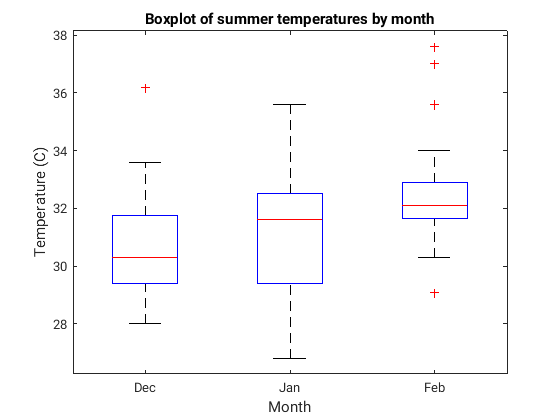
\includegraphics[scale=0.8]{boxplot.png}
\caption{Boxplot of monthly temperature spread over the summer months of 2016-2017}
\end{figure}

\newpage
\section{Understanding error messages}
TL;DR: \textbf{Copy and paste your error message into a web browser, click on the most pertinent link. This will almost surely take you to a forum with the best responses first.}\\

Error messages are not to be ignored. They will usually tell you why the computation failed. You might need some skills to understand what went wrong in the lead up to the failure. Below are some common error messages. See if you can understand them.\\

\begin{lstlisting}
>> b = a + 4.2;
% Undefined function or variable 'a'.

>> t_range = [0 1]; y0 = 0.01;
>> y = ode45(@myUndefinedFunction, t_range, y0);
%Undefined function or variable 'myUndefinedFunction'.

%Error in odearguments (line 87)
%f0 = feval(ode,t0,y0,args{:});   % ODE15I sets args{1} to yp0.

%Error in ode45 (line 115)
%    odearguments(FcnHandlesUsed, solver_name, ode, tspan, y0, options, varargin);


>> A_matrix = [1 2 3; 4 5 6; 7 8 9];
>> b_vector = [1 2];
>> A_matrix * b_vector;
%Error using  * 
%Inner matrix dimensions must agree.


\end{lstlisting}

If you're having trouble with the error message written to the console, copy it and paste it into your favourite search engine. You will often find results from Stack Exchange or Mathworks fora at the top of the results. These are the best places to start. Make sure you just include the important parts. For example, if the error message is complaining about something done in your custom function called \texttt{COD\_calculator}, remove any reference to your function's name when you paste the error message into the browser. 

\end{document}